%%=============================================================================
%% Methodologie
%%=============================================================================

\chapter{\IfLanguageName{dutch}{Methodologie}{Methodology}}%
\label{ch:methodologie}


\lstset{
    language=yaml
    basicstyle=\ttfamily,
    columns=fullflexible,
    frame=single,
    breaklines=true
}
%% TODO: Hoe ben je te werk gegaan? Verdeel je onderzoek in grote fasen, en
%% licht in elke fase toe welke stappen je gevolgd hebt. Verantwoord waarom je
%% op deze manier te werk gegaan bent. Je moet kunnen aantonen dat je de best
%% mogelijke manier toegepast hebt om een antwoord te vinden op de
%% onderzoeksvraag.

\section{title}
trying to run nginx on kubernetes with example from https://blog.meain.io/2020/dynamic-reverse-proxy-kubernetes/

\begin{lstlisting}
apiVersion: apps/v1
kind: Deployment
metadata:
    name: nginx
    labels:
        app: nginx
spec:
    selector:
        matchLabels:
            app: nginx
    replicas: 1
    template:
        metadata:
            labels:
                app: nginx
        spec:
            containers:
                - name: nginx
                    image: nginx:alpine
                    ports:
                        - containerPort: 80
                    volumeMounts:
                        - name: nginx-config
                            mountPath: /nginx.conf
                            subPath: nginx.conf
                    volumes:
                        - name: nginx-config
                            configMap:
                                name: confnginx
---
apiVersion: v1
kind: Service
metadata:
    name: nginx
    labels:
        name: nginx
spec:
    selector:
        app: nginx
    ports:
        - protocol: TCP
          port: 80
          targetPort: 80
          name: nginx
    type: LoadBalancer
---
apiVersion: v1
kind: ConfigMap
metadata:
    name: confnginx
data:
    nginx.conf: |
        user  nginx;
        worker_processes  1;
        error_log  /var/log/nginx/error.log warn;
        pid        /var/run/nginx.pid;
        events {
            worker_connections  1024;
        }
        http {
            include       /etc/nginx/mime.types;
            default_type  application/octet-stream;
            log_format  main  '$remote_addr - $remote_user [$time_local] "$request" '
            '$status $body_bytes_sent "$http_referer" '
            '"$http_user_agent" "$http_x_forwarded_for"';
            access_log  /var/log/nginx/access.log  main;
            sendfile        on;
            keepalive_timeout  65;
            server {
                listen 80;
                
                resolver kube-dns.kube-system.svc.cluster.local valid=5s;
                
                location /healthz {
                    return 200;
                }
            }
        }
\end{lstlisting}

worked until trying to figure out what every is doing pricicely and to configurate nginx because of this screen
\newline
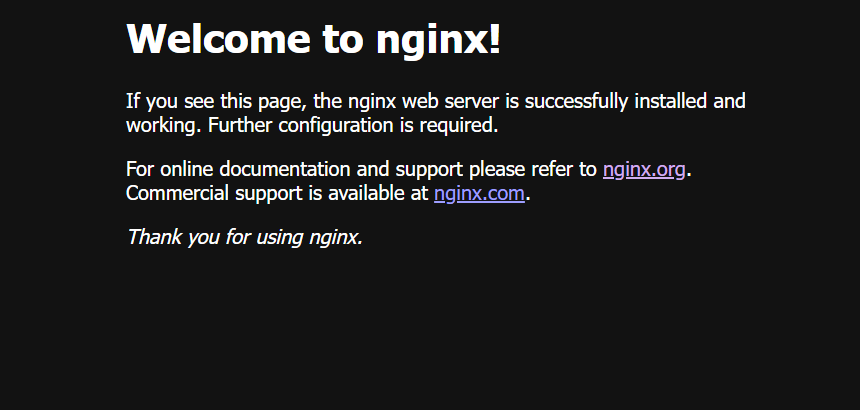
\includegraphics{nginx welcom screen.png}

learnt later that how to enable external ip for service you need to add "type: LoadBalancer" because "The load balancer tracks the availability of pods with the Kubernetes Endpoints API. When it receives a request for a specific Kubernetes service, the Kubernetes load balancer sorts in order or round robins the request among relevant Kubernetes pods for the service." %(https://avinetworks.com/glossary/kubernetes-load-balancer/#:~:text=The%20load%20balancer%20tracks%20the,Kubernetes%20pods%20for%20the%20service.)
%(https://stackoverflow.com/questions/41509439/whats-the-difference-between-clusterip-nodeport-and-loadbalancer-service-types)

Hoe met 1 yaml file kunnen verschillnde user voor verschillende pods doen environment variables??? TODO


\subsubsection{Annotations or labels}


You can use either labels or annotations to attach metadata to Kubernetes objects. Labels can be used to select objects and to find collections of objects that satisfy certain conditions. In contrast, annotations are not used to identify and select objects. The metadata in an annotation can be small or large, structured or unstructured, and can include characters not permitted by labels.


\subsubsection{clusterip}


Choosing your own IP address
You can specify your own cluster IP address as part of a Service creation request. To do this, set the .spec.clusterIP field. For example, if you already have an existing DNS entry that you wish to reuse, or legacy systems that are configured for a specific IP address and difficult to re-configure.

The IP address that you choose must be a valid IPv4 or IPv6 address from within the service-cluster-ip-range CIDR range that is configured for the API server. If you try to create a Service with an invalid clusterIP address value, the API server will return a 422 HTTP status code to indicate that there's a problem.
\newline

probeer authenticatie toe te voegen maar probeer eerst op een pagina te komen om dan te blockeren zodat ik the authenticatie can doen maar krijg 404 code omdat in pod er gezocht word op de default plaats van nginx "/usr/share/nginx/html/REQUEST" en probeer nu gewoon 200 code terug te geven of index.html filetje

het kwam door dat ik mijn volumes en mounted volumes niet goed had ingesteld voor nginx ze werden niet goed vervangen en ik had het doel van mounted volumes en volumes in omgewisselt

nieuwe yaml file met authenticatie
\begin{lstlisting}
apiVersion: v1
kind: ConfigMap
metadata:
    name: confnginx
data:
    nginx.conf: |
        user  nginx;
        worker_processes  1;

        error_log  /var/log/nginx/error.log warn;
        pid        /var/run/nginx.pid;

        events {
            worker_connections  1024;
        }
        http {
            include       /etc/nginx/mime.types;
    
            default_type  application/octet-stream;
    
            log_format  main  '$remote_addr - $remote_user [$time_local] "$request" '
            '$status $body_bytes_sent "$http_referer" '
            '"$http_user_agent" "$http_x_forwarded_for"';
    
            access_log  /var/log/nginx/access.log  main;
    
            sendfile        on;
    
            keepalive_timeout  65;
    
            server {
                listen 80;
                listen [::]:80;
                server_name localhost;
        
                index index.html;
        
                resolver kube-dns.kube-system.svc.cluster.local valid=5s;
        
                auth_basic "Access restricted";
                auth_basic_user_file /etc/nginx/password.conf;
        
                location / {
                root /usr/share/nginx/html;
                index index.html index.htm;
                }
        
            }
        }
    password.conf: |
        bekdestester:$6$8tHKH5TSh$FbIquguOZIvMzc52APCPGaVUq8N2vhmQlsxfV7PIiVJNTzKWRRrkHqbFsY4DfTqHNZNcejO.dOGpgdwPzzNG80
        firelay:$6$2SpUcpng9JqnLOO9$5oLMFZOQdNjqTeUBGW8Tf0.mw0unAlVuqh8Dt4cHpsa4EzAMDTL1ylKSNErURDO3QqN0f/Gdyg5sUhYhWKYCu.
    index.html: |
        <html>
        <body>
        <p>Some secrets:</p>
        <ul>
        <li><pre>username: .Data.username </pre></li>
        <li><pre>password: .Data.password </pre></li>
        </ul>
        </body>
        </html>
---
apiVersion: apps/v1
kind: Deployment
metadata:
    name: nginx
    labels:
        app: nginx
spec:
    selector:
        matchLabels:
            app: nginx
    replicas: 1
    template:
        metadata:
            labels:
                app: nginx
        spec:
            containers:
                - name: nginx
                    image: nginx:alpine
                    ports:
                        - containerPort: 80
                    volumeMounts:
                        - mountPath: /etc/nginx/nginx.conf
                            subPath: nginx.conf
                            readOnly: true
                            name: nginx-conf
                        - mountPath: /etc/nginx/password.conf
                            subPath: password.conf
                            readOnly: true
                            name: password-conf
                        - mountPath: /usr/share/nginx/html # mount nginx-htmlroot volume to /usr/share/nginx/html
                            readOnly: true
                            name: nginx-htmlroot
                    volumes:
                        - name: nginx-conf
                            configMap:
                                name: confnginx
                                items:
                                    - key: nginx.conf
                                      path: nginx.conf
                        - name: password-conf
                            configMap:
                                name: confnginx
                                items:
                                    - key: password.conf
                                      path: password.conf
                        - name: nginx-htmlroot
                            configMap:
                                name: confnginx
                                items:
                                    - key: index.html
                                      path: index.html
---
apiVersion: v1
kind: Service
metadata:
    name: nginx
    labels:
        name: nginx
spec:
    selector:
        app: nginx
    ports:
        - protocol: TCP
          port: 80
          targetPort: 80
          name: nginx
    type: LoadBalancer
\end{lstlisting}